\subsection{Nonlinear Invariant Cryptanalysis}

\renewcommand{\TITLE}{\it Nonlinear Invariant Cryptanalysis}

\begin{frame}[t]
\vspace{1.25cm}
\CurTitle{}

\Center{
    \textcolor{blue}{Properties} of messages that are \textcolor{green!70!black}{preserved} through encryption
}

\vspace{-0.5cm}

\only<2>{\Center{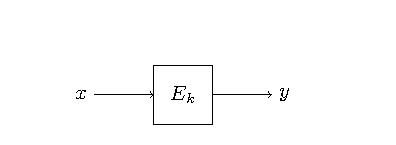
\includegraphics[height=3cm]{invariant1.pdf}}}
\only<3>{\Center{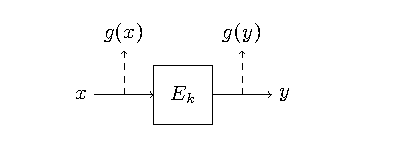
\includegraphics[height=3cm]{invariant2.pdf}}}
\only<4>{\Center{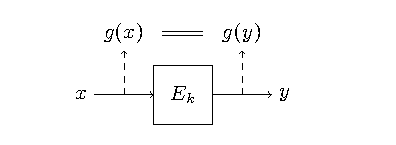
\includegraphics[height=3cm]{invariant3.pdf}}}
\only<5>{\Center{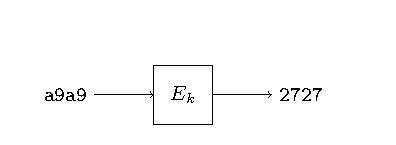
\includegraphics[height=3cm]{invariant4.pdf}}}
\only<6>{\Center{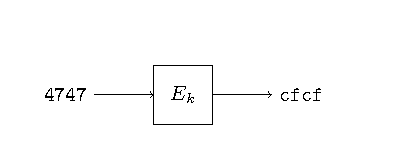
\includegraphics[height=3cm]{invariant5.pdf}}}
\end{frame}


\begin{frame}[t]
\CreditsTikz{}
\CurTitle{}

\Center{
\hspace*{1.75cm}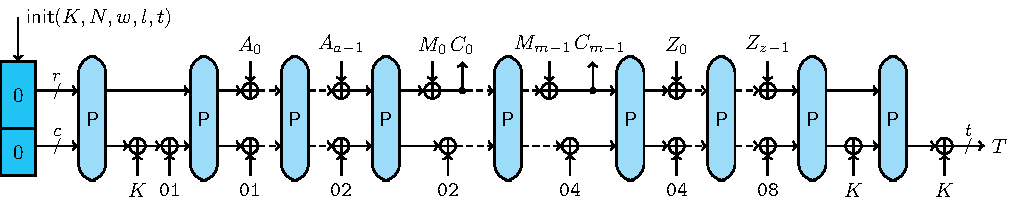
\includegraphics[width=0.85\linewidth]{norx_sponge_serial_v3.pdf}
}

\Block{4cm,4cm}{5cm}{
    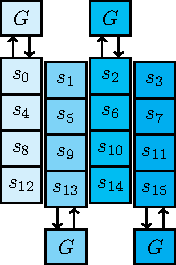
\includegraphics[width=2.5cm]{norx_G_col.pdf}
}
\Block{8cm,4cm}{5cm}{
    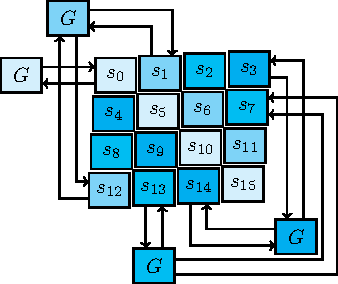
\includegraphics[width=4.5cm]{norx_G_diag.pdf}
}

\vspace{3.75cm}

\Center{
    \Large Analysis of the NORX Authenticated Encryption
}
\end{frame}


\begin{frame}[t]
\CurTitle{}

\vspace{1cm}

$$
\begin{bmatrix}
0 & 0 & 0 & 0 & 1 & 1 & 1 & 1 & 1 & 1 & 1 \\
0 & 1 & 1 & 1 & 0 & 0 & 0 & 1 & 1 & 1 & 1 \\
1 & 0 & 1 & 1 & 0 & 1 & 1 & 0 & 0 & 1 & 1 \\
1 & 1 & 0 & 1 & 1 & 0 & 1 & 0 & 1 & 0 & 1 \\
1 & 1 & 1 & 0 & 1 & 1 & 0 & 1 & 0 & 0 & 1 \\
\end{bmatrix}
$$

\vspace{0.5cm}

\Center{
    \Large Theoretical study of linear layers \\
    preserving degree-$d$ invariants
}
\end{frame}


\begin{frame}[t]
    \CurTitle{}
    
    \nocitepartii{mybibNORX}
    \nocitepartii{mybibNLI}
    \bibliographystylepartii{unsrt}
    \Block{3cm,2.5cm}{10cm}{
        \bibliographypartii{mybiblio.bib}
    }
\end{frame}